\documentclass[11pt]{article}
\usepackage{ctable,microtype,natbib,amsmath,amssymb,fullpage,graphicx}
\usepackage{siunitx}
\usepackage{cleveref}
\usepackage{keyval,kvoptions,fancyvrb,float,ifthen,calc,ifplatform,pdftexcmds,etoolbox,lineno}
\usepackage[utf8]{inputenc}
\usepackage{color}
\usepackage[danish]{babel}
\usepackage[left=25mm, right=25mm, top=25mm, bottom=25mm]{geometry}
\usepackage{lastpage}
\usepackage{amsthm}
\setlength\parindent{0pt}
\usepackage{fancyhdr}
\usepackage{dcolumn}
\usepackage{minted} 
\usepackage{setspace}

\onehalfspacing

\title{Hardware}
\author{Christian Bondesen - 201511621}

\begin{document}
\maketitle
\section{Design: }
I design fasen af hardwaren er der udarbejdet et udfra arkitekturen et design af hvert enkelt HW-blok. Her er der tale om 4 hardware dele, 2 gange X-10 Zero-cross, X-10 modtager og X-10 Generator. Der er analyseret udfra ``AN236 Application Note'' og ``introduktion til 2. Semesterprojekter'', er der udarbejdet følgende hardwareblok for Smart Morning System: 
\begin{figure}[!h]
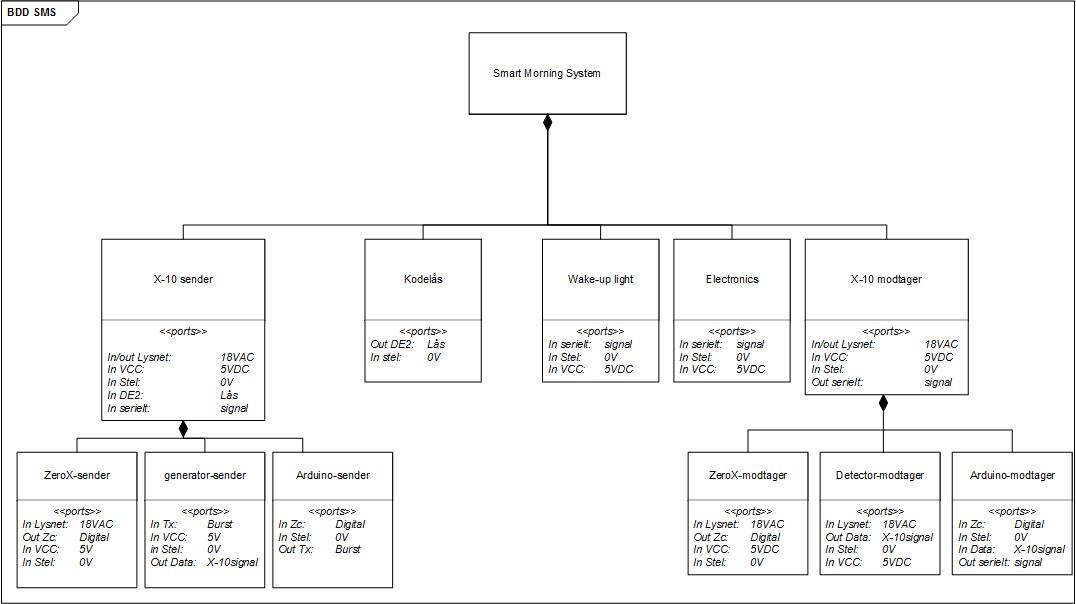
\includegraphics[scale = 0.6, ]{Bdd-sms}
\caption{BDD af Smart Morning System, med de forskellige ports og parts}
\end{figure} \\
Det er tiltænkt at enhederne fra systemet skulle kunne kommunikere med hinanden via X-10 protokolen. Det er muligt gjort ved at designe følgende hardware dele i blokke. Disse blokke og deres funktionalitet vil i følgende afsnit blive beskrevet, da de er centrale for systemet. 
\subsection{X-10 Zero-cross: }
Herunder ses et billede af en simulering for X-10 Zero-cross, formålet for denne hardwaredel er at sende et 5V signal til Mega2560 når netspændingen passerer 0V på lysnettet sinussignal:
\begin{figure}[!h]
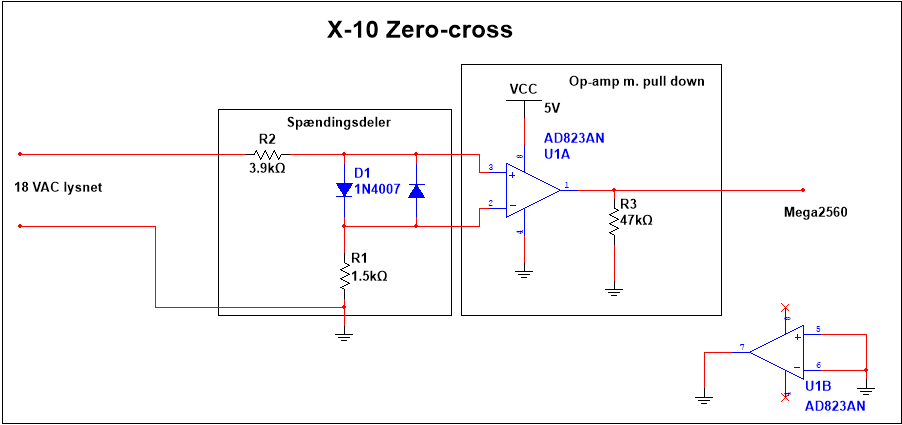
\includegraphics[scale = 0.7]{Zero-cross-ms}
\caption{Multism billede af X-10 Zero-cross m. specifikke komponent værdier}
\end{figure}\\
Med udgangspunkt i ``AN236 Application Note'' blev der lavet en spændingsdeler, bestående af en modstand på 3,9k$\Omega$, 2 dioder og en modstand på 1,5k$\Omega$. Mega2560 kan ikke tage 18VAC fra lysnettet, der af er der laver følgende beregninger for at undgå for høj spænding til Microcontrolleren: 
\begin{figure}[!h]
\centering
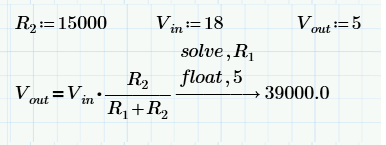
\includegraphics[scale = 1]{udregning-af-spandingsdeler}
\caption{Udregning af spændingsdeler modstand}
\end{figure}\\
Diodernes funktion for spændingsdeleren er at sikre at strømmen ikke over går 5V eller -5V. På spændingsdeleren er der en Op-amp der sikre at Mega2560 altid ved få 5V så der ikke opstår falske nulgennemgange i vores kredsløb. Dvs. den er designet til at sende signal i det spændingen er tilpas påtrykt op-ampen. Her er tilføjet en pulldown modstand. Systemet er designet som på figur 2. Lysnettet sendes ind gennem spændingsdeleren giver en spænding på 5VAC der løber gennem Op-ampen og ind i Mega2560.

\subsection{X-10 Modtager: }
X-10 Modtageren har til opgave at modtage et lysnettet og frasortere de 120kHz burst der er sendt ud på lysnettet. Herunder ses et diagram over X-10 modtagerens forskellige dele i sammenhæng med hinanden:
\begin{figure}[!h]
\centering
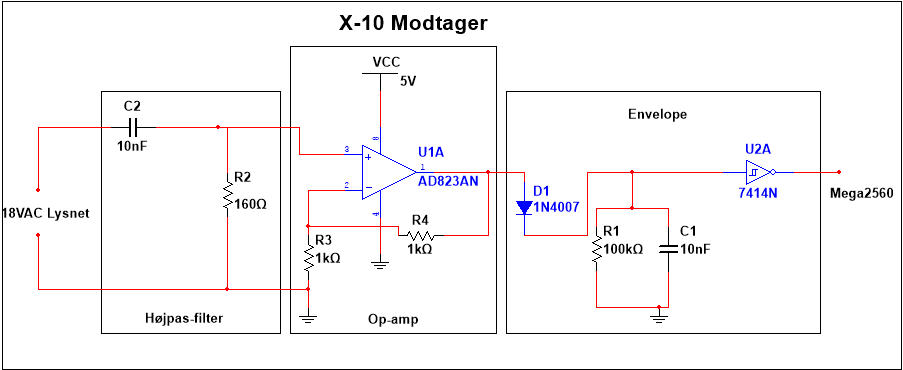
\includegraphics[scale = 0.7]{X-10modtager}
\caption{Diagram over X-10 modtager m. specifikke komponenter}
\end{figure}\\
X-10 Modtager består af et højpasfilter, en forstærkende Op-amp og en envelope-detector. Disse dele er fundet frem til ved hjælp af X-10 protokolen i ``AN236 Application Note''. Der er valgt et højpas filter, da vi kun har interesse for de højfrekvenser der er sendt ud på lysnettet. Filteret er et simpelt RC-filter hvor komponentværdierne er udregnet på følgende måde:
\begin{figure}[!h]
\centering
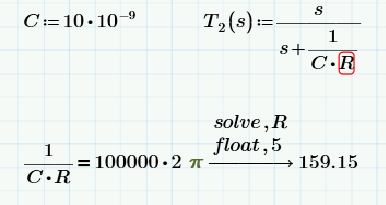
\includegraphics[scale = 0.8]{Hojspas-modtager}
\caption{Udregning af højpasfilter for X-10 Modtager}
\end{figure}\\
Der er valgt en kondensator på forhånd udfra de komponenter der var tilrådighed i komponentlageret. Heraf blev der sat en cut-off frekvens på 100kHz for at sikre at alle frekvenser på 120kHz ville gå igennem. Heraf fik vi højpasfilteret. \\
Den næste del i X-10 Modtageren har vi en forstærkende Op-amp, der blev erfaret at forstærkningen var nødvendig da spændingen efter ikke var stor nok for at gå igennem dioden. Herefter går spændingen direkte gennem en diode der sikre at strømmen kun løber en vej. Udfra X-10 protokolen fra ``AN236 Application Note'' er der lavet en envelope-detector med en inverterende Schmidt-trigger. Envelope-detectoren har til opgave at samle 120kHz burst'ne til et enkelt lavt signal. Dette signal aflæses så af Mega2560. Envelopen er bygget op af en kodensator og en modstand i serie med en diode. 

\subsection{X-10 Generator}
X-10 Generator har til formål at overlejre et 120kHz burst ud på lysnettet når der ønskes at sendes et scenarie. Herunder ses et digram over de forskellige komponenter og design der er udarbejdet til X-10 Generatoren:
\begin{figure}[!h]
\centering
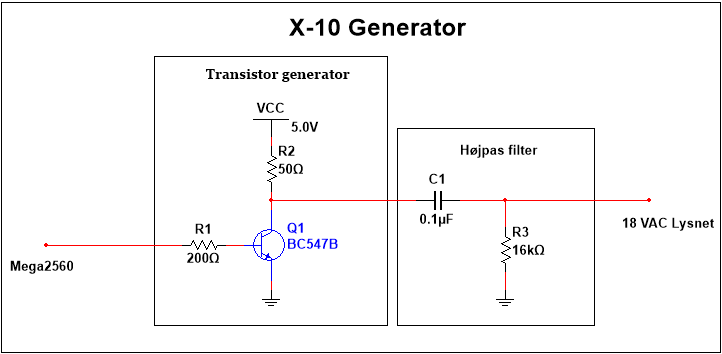
\includegraphics[scale = 0.9]{X10-generator-ms}
\caption{Diagram af generator med specifikke komponenter}
\end{figure}\\
Efter analyse af X-10 prokolen fra ``AN236 Application Note'' og supplerende videoer fra suppleringsmaterialet. Blev der fundet frem til at generatoren skulle sende 120kHz burst der overlejres til lysnettet. Der er derfor valgt en transistor der er i stand til skifte tilstand med en frekvens på 120kHz. Der er derfor valgt en BC547B. For at beskytte komponentet er der formodstande på der stadig gør det muligt for transistoren at detektere et højt signal. Transistoren er efterfulgt af et højpasfilter der tilsvarende det der er brugt på X-10 Modtageren. Filteret er dog skaleret op med en skaleringsfaktor på 100, udregningen ses herunder:
\begin{figure}[!h]
\centering
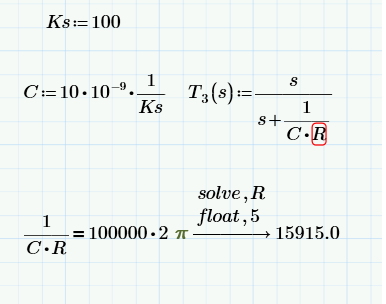
\includegraphics[scale = 0.5]{udregningHPgenerator}
\caption{Udregning for højpasfilter for X-10 Generator med skalering}
\end{figure}\\
Der blev valgt at skalere komponenterne da lageret var løbet tør for de komponenter der tidligere var anvendt.



\end{document}